\chapter{微型无人机集群测距与自主导航原型系统}


\section{ 引言}

随着微型无人机在复杂环境中的应用需求不断提升，单机自主导航已难以满足高效率、高鲁棒性的任务要求，多无人机集群协同逐渐成为研究热点。
然而，在实际应用中，受限于微型无人机平台的计算资源、通信带宽以及传感能力，实现集群级别的稳定测距、可靠定位以及自主导航仍面临诸多挑战，尤其是在复杂未知环境下，如何构建一个具备完整闭环能力的原型系统，是从算法研究走向工程落地的关键问题。

针对上述问题，本文在前几章的研究基础上，进一步开展微型无人机集群测距与自主导航原型系统的设计与实现工作。
第三章围绕集群相对定位问题，提出了一种基于UWB的自适应协同定位方法，通过鲁棒测距协议与期望最大化算法相结合，实现了多无人机环境下稳定且高精度的相对定位；
第四章则针对复杂环境中的自主导航问题，基于分布式强化学习框架，提出了自适应风险倾向隐式分位网络算法，有效提升了无人机在低概率高风险场景下的决策安全性与鲁棒性，并完成了模型训练与嵌入式部署。

在此基础上，本章面向系统级集成与真实场景验证，构建了一个完整的微型无人机集群自主导航原型系统。
该系统以Crazyflie 2.1微型无人机为核心平台，结合Adhoc Deck扩展板，实现机载计算、通信与感知能力的集成。
在系统架构上，采用“感知—定位—决策—控制”的分层设计思路，其中领导者无人机基于第四章提出的导航算法实现自主路径规划与避障飞行，而跟随无人机则依托第三章的协同定位方法获取相对位姿信息，并结合简化避障策略完成编队跟随与局部避碰，从而实现集群层面的协同运动。

同时，为保证系统在实际运行中的稳定性与实时性，本文进一步设计并实现了完整的软硬件体系，包括嵌入式模型部署、无人机内部通信机制、飞行控制接口以及外部监控系统等关键模块，并对系统运行流程与部署方案进行了系统化设计。
通过构建真实飞行实验环境，对所提出的集群测距与自主导航方法进行了综合验证。

实验结果表明，所构建的原型系统能够在资源受限的微型无人机平台上稳定运行，实现多无人机之间的可靠测距与协同定位，并支持领航-跟随模式下的自主导航与避障飞行，验证了本文所提方法在实际复杂环境中的可行性与有效性。

\section{系统硬件组成}
\begin{figure}[htbp]
  \centering
  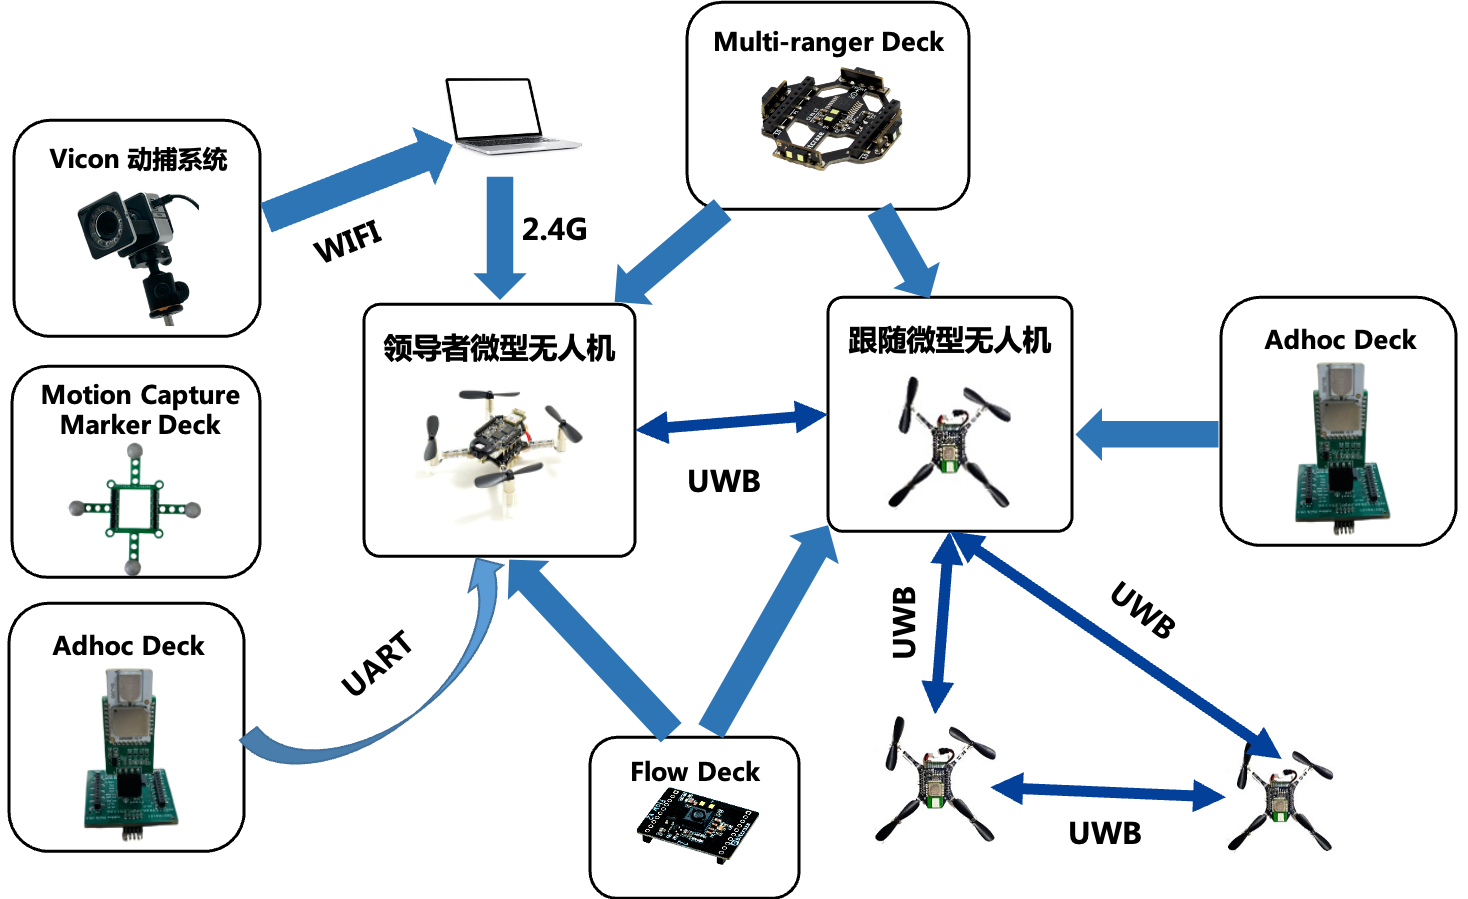
\includegraphics[width=.8\linewidth]{figures/content/chapter5/硬件架构.png}
  \caption{原型系统硬件架构}
  \label{fig:5_1}
\end{figure}

本文构建的微型无人机集群自主导航系统的硬件架构如图\ref{fig:5_1}，整体由外部监控系统、领导者无人机、跟随者无人机以及多种计算或传感器扩展模块组成。

在外部系统部分，基于 Vicon 动作捕捉系统 与 Motion Capture Marker Deck 实现高精度位姿获取，并通过服务器经 WiFi 将位置信息发送至电脑端。
同时，电脑端通过Crazy Radio PA的2.4GHz 无线链路与无人机通信，作为导航传入的必要数据。

在无人机平台方面，系统采用“领导者—跟随者”分层结构：领导者无人机搭载 Adhoc Deck 与 其他的传感器扩展模块，其中 Adhoc Deck 提供嵌入式计算能力与UWB通信，用于运行协同定位算法与自主导航；
其他的传感器模块用来为导航传入必要的输入数据。
跟随无人机主要依赖 UWB 模块进行相对测距与定位，通过与领导者及其他无人机之间的 UWB 通信，实现分布式协同定位与编队跟随。
\subsection{无人机平台}
\begin{figure}[htbp]
    \centering
    \subfloat[Adhoc Deck]{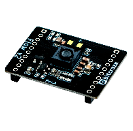
\includegraphics[width=.23\textwidth]{figures/content/chapter5/FlowDeck.png}}
    \quad
    \subfloat[Flow Deck]{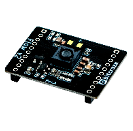
\includegraphics[width=.23\textwidth]{figures/content/chapter5/FlowDeck.png}}
    \quad
    \subfloat[Multi-ranger Deck]{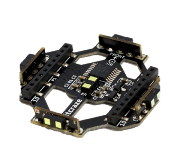
\includegraphics[width=.23\textwidth]{figures/content/chapter5/MultirangDeck.png}}
    \quad
    \subfloat[Motion Capture Marker Deck]{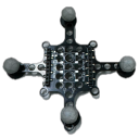
\includegraphics[width=.23\textwidth]{figures/content/chapter5/viconDeck.png}}
    \caption{领导者无人机硬件模块组成}
    \label{fig:5_2}
    \end{figure}
如图\ref{fig:5_2}所示，领岛无人机搭载了多种功能扩展板，用于实现感知、计算与定位等关键功能，具体包括 Adhoc Deck、Flow Deck、Multi-ranger Deck 以及 Motion Capture Marker Deck。

其中，Adhoc Deck 是系统的核心计算模块，基于嵌入式处理器构建，负责运行本文提出的协同自主定位于自主导航算法，实现机载实时决策。
同时，该扩展板支持外设接口扩展，可集成 UWB 模块，从而具备测距与通信能力，使领导者无人机既能够执行导航任务，又能够参与集群间的相对定位与信息交互。
Flow Deck 主要用于提供对地速度与高度信息，其通过光流传感器与 ToF 距离传感器实现对无人机平面运动速度及离地高度的估计，在无外部定位系统的情况下可辅助飞行稳定与状态估计。
Multi-ranger Deck 集成多个方向的距离传感器，可实时获取无人机前、后、左、右及上方的障碍物距离信息，为自主导航算法提供环境感知输入，从而支持局部避障决策。
Motion Capture Marker Deck 搭载反光标记点，用于配合外部动捕系统获取高精度位姿信息，为导航模型提供输入的数据。


\begin{figure}[htbp]
    \centering
    \subfloat[UWB Deck]{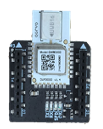
\includegraphics[width=.23\textwidth]{figures/content/chapter5/UWBDeck.png}}
    \quad
    \subfloat[Flow Deck]{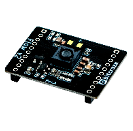
\includegraphics[width=.33\textwidth]{figures/content/chapter5/FlowDeck.png}}
    \quad
    \subfloat[Multi-ranger Deck]{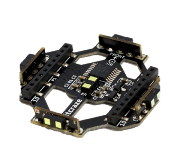
\includegraphics[width=.33\textwidth]{figures/content/chapter5/MultirangDeck.png}}
    \caption{跟随者无人机硬件模块组成}
    \label{fig:5_3}
    \end{figure}
如图\ref{fig:5_3}所示，跟随无人机主要搭载 UWB Deck、Flow Deck 以及 Multi-ranger Deck，以实现相对定位与局部避障等功能。

其中，UWB Deck 是跟随无人机实现协同定位的核心模块。该扩展板基于 UWB 芯片，能够与领导无人机及其他跟随者之间进行高精度测距与数据交互。通过构建多节点间的测距网络，并结合第三章提出的自适应协同定位算法，跟随无人机能够实时获取自身在集群中的相对位姿信息，从而实现对领导者的稳定跟随。
Multi-ranger Deck 集成多方向距离传感器，用于实时感知周围障碍物距离信息。
跟随无人机在执行编队跟随任务的同时，可基于该模块提供的环境感知信息实现局部避障与避碰，从而提升系统在复杂环境中的安全性。

领导者与跟随者无人机搭载各种扩展版的最终图\ref{fig:5_4}所示。
\begin{figure}[htbp]
    \centering
    \subfloat[领导者无人机]{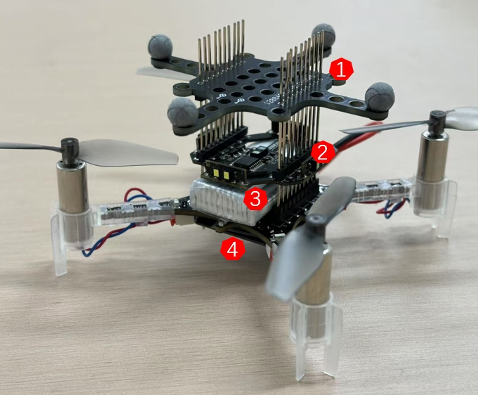
\includegraphics[width=.45\textwidth]{figures/content/chapter5/领导者图片.png}}
    \quad
    \subfloat[跟随者无人机]{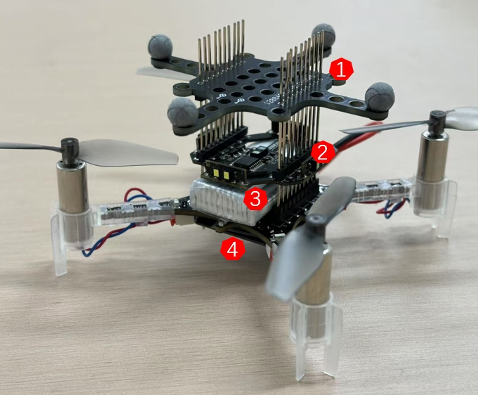
\includegraphics[width=.45\textwidth]{figures/content/chapter5/领导者图片.png}}
    \caption{无人机集群自主导航系统}
    \label{fig:5_3}
\end{figure}
\subsection{外部监控平台}
外部监控平台主要由 Vicon 动作捕捉系统 与 Crazyradio PA 无线通信模块 构成，用于实现无人机状态获取与飞行指令下发。

\begin{figure}[htbp]
  \centering
  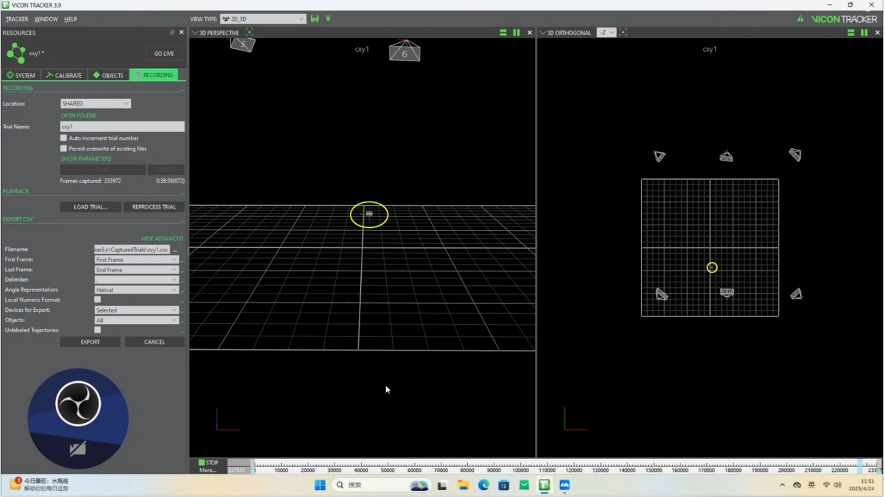
\includegraphics[width=.7\linewidth]{figures/content/chapter5/vicon平台.png}
  \caption{vicon 监控平台}
  \label{fig:5_4}
\end{figure}

其中，Vicon 动作捕捉系统 通过在无人机上安装 Motion Capture Marker Deck，利用多台红外摄像机对标记点进行实时捕捉与三维重建，从而获取无人机在全局坐标系下的高精度位姿信息。该系统具有厘米级甚至毫米级的定位精度与较高的更新频率，可为算法开发与实验验证提供可靠的“真值”参考。

在安装 Motion Capture Marker Deck 后，需要对动作捕捉系统进行校准，以确保定位精度与系统稳定性。具体步骤如下：

\begin{enumerate}
    \item 准备工作：  
    确保 Vicon 系统硬件（如摄像机、反光标记球等）已正确安装并连接正常，相关软件已完成安装并成功启动。同时，将反光球合理粘贴在被捕捉对象（如人体或无人机）关键位置，以保证后续识别的稳定性与准确性。

    \item 摄像机聚焦：  
    打开 Vicon 系统软件，进入摄像机调试与聚焦模块。按照软件提示依次对各个摄像机进行校准，使各摄像机视野中不存在多余光斑（建议在避光环境下进行）。当每个摄像机画面中的标记点均显示为蓝色时，表明摄像机校准完成。

    \item 空间坐标校准：  
    使用校准工具（带反光球的标定棒）在整个捕捉空间内移动，构建全局空间坐标系。系统根据多摄像机采集的数据，计算空间中各标记点的位置关系，从而完成对捕捉空间范围及坐标系的标定。

    \item 建立刚体模型：  
    检查粘贴在 Motion Capture Marker Deck 上的反光球是否牢固且分布合理。将无人机置于捕捉空间内，系统对反光球的标记点进行识别与建模。通常至少需要三个非共线标记点才能建立刚体模型，本实验中共使用四个反光球进行建模，最终建立的刚体模型如图~\ref{fig:5_4} 所示。

    \item 数据检查：  
    校准完成后，进行简单的动作捕捉测试，观察系统输出的数据是否连续、平滑，是否存在异常跳变或数据丢失现象。如发现问题，应返回对应步骤重新进行校准，以确保系统性能满足实验要求。
\end{enumerate}

Crazyradio PA 是用于连接上位机与无人机的 2.4GHz 无线通信模块。其通过 USB 接口与计算机相连，并基于 Crazyflie 通信协议（CRTP）与无人机建立稳定的数据链路。
上位机可通过 Crazyradio PA 向领导者无人机发送飞行控制指令，同时接收无人机回传的状态信息，实现对系统运行过程的实时监控与参数调节。

\section{系统软件模块}
本文构建的微型无人机集群测距与自主导航原型系统在软件层面采用分层解耦与模块化设计方法，整体由单机功能模块、集群协同功能模块以及算法支撑模块三部分组成，并围绕“感知—定位—决策—控制—通信”的处理流程构建完整闭环。

在单机层面，系统根据功能角色的不同，将无人机划分为领导者与跟随者两类节点，其软件架构在统一框架下进行差异化设计。

对于领导者无人机，其模块层主要包括飞行控制模块、自主导航模块以及协同定位模块。其中，飞行控制模块位于系统底层，负责接收上层控制指令并完成姿态与速度的闭环控制；自主导航模块作为核心决策单元，基于强化学习模型输出无人机在复杂环境中的运动决策，实现路径规划与动态避障；协同定位模块则参与集群测距与状态估计过程，为系统提供相对位置信息支撑。各模块之间通过统一的数据接口进行交互，使导航决策能够平滑映射至底层控制执行。

对于跟随无人机，其模块层包括飞行控制模块、协作通信定位模块以及局部避障模块。其中，协作通信定位模块基于 UWB 测距与信息交互机制，结合分布式定位算法实现无人机间的相对位姿估计；局部避障模块利用机载传感器信息对周围环境进行感知，并在跟随过程中对潜在碰撞进行规避；飞行控制模块则根据定位结果与跟随策略输出控制量，实现对领导者无人机的稳定跟随。相比领导者，跟随者不直接参与全局路径规划，而侧重于协同感知与局部决策。

在集群层面，系统进一步抽象为两个核心子系统，即集群定位飞行任务子系统与自主导航任务子系统。其中，集群定位飞行任务子系统主要负责无人机之间的测距、通信以及协同定位，对应本文第三章提出的自适应协同定位方法；自主导航任务子系统则由领导无人机主导，负责在复杂未知环境中的路径规划与避障决策，对应第四章提出的强化学习导航算法。两个子系统相互协同，共同支撑集群飞行任务的完成。

在数据流层面，系统整体运行过程可描述为：环境感知与测距数据首先由各类传感器与通信模块获取，经协同定位模块融合得到无人机状态信息；
随后，领导者无人机基于自主导航模块输出控制决策，跟随无人机根据相对位姿与跟随策略生成控制指令；最终，飞行控制模块将高层指令转换为底层执行信号，驱动无人机完成相应运动。同时，通信模块贯穿整个系统，实现无人机之间以及无人机与上位机之间的数据交互。
在上述整体架构基础上，针对前文尚未详细说明的关键功能模块，本文进一步对跟随避障算法、通信模块以及飞行控制模块进行补充说明。
\begin{figure}[htbp]
  \centering
  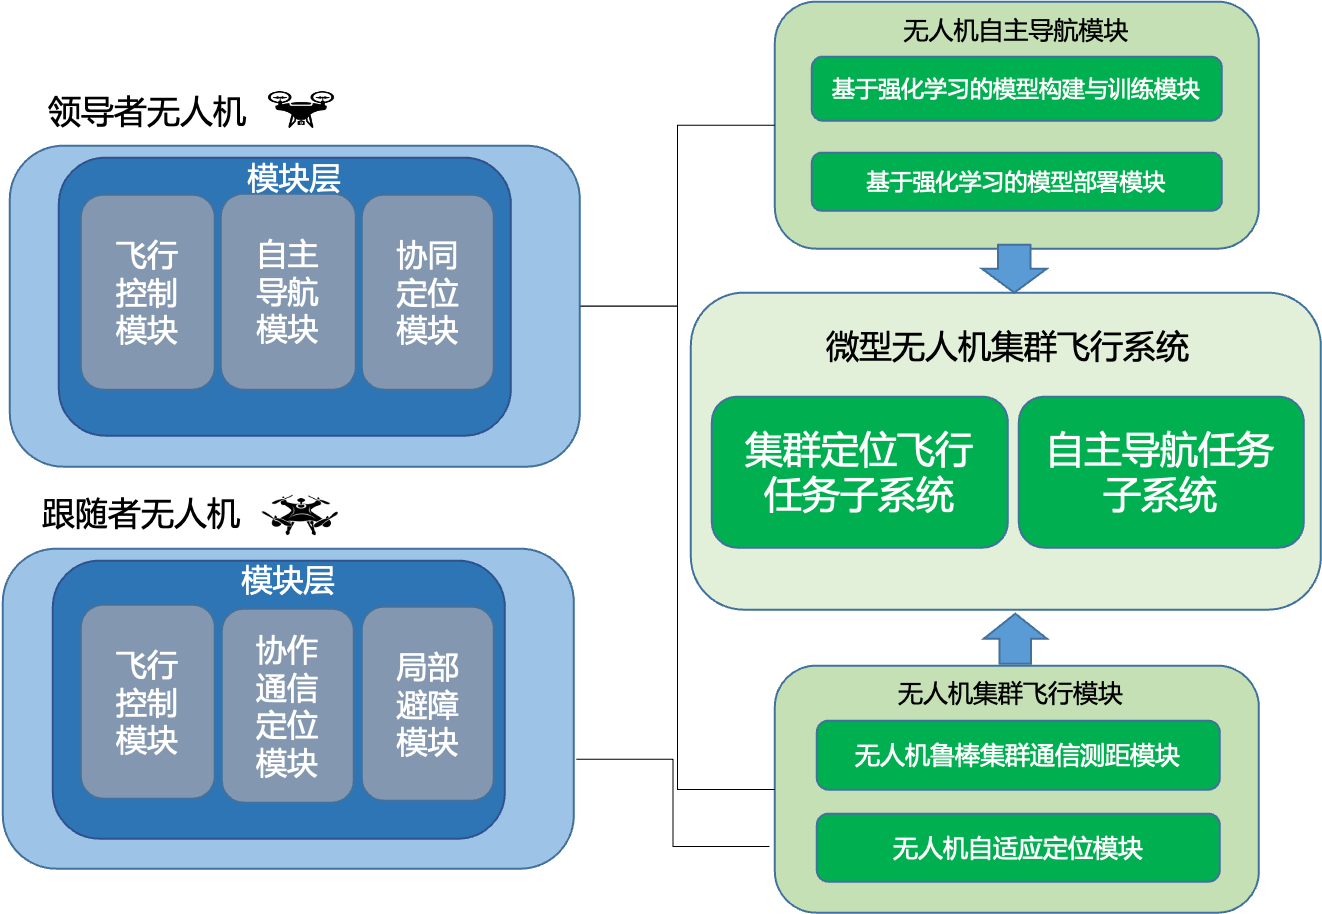
\includegraphics[width=.6\linewidth]{figures/content/chapter5/软件架构.png}
  \caption{系统软件架构}
  \label{fig:5_5}
\end{figure}
\subsection{跟随与避障模块}
在多无人机编队飞行中，每架无人机都有其在领导者坐标系下的预定位置。
为了简化问题，我们将0号无人机设置为编队中的领导者，因此其预定位置被设为坐标系原点。
首先，仅考虑编队保持任务时，第$i$架无人机的速度控制律采用经典PID形式\cite{knospe2006pid}表示为：
\begin{equation}
\boldsymbol{v}_{i}=k_{p} \boldsymbol{e}_{i 0}+k_{d} \dot{\boldsymbol{e}}_{i 0}+k_{i} \int \boldsymbol{e}_{i 0} d t
\end{equation}
其中，$\boldsymbol{e}_{i 0}$为领导者与跟随着的相对位置偏差，也就是预定位置和实际位置之间的差异。

对于无人机周边的外界障碍物的碰撞避免，我们假设无人机可以通过传感器得知障碍物相对机体坐标系下的具体位置$ \boldsymbol{p}_{i}^{o b s}=\left(x_{i}^{o b s}, y_{i}^{o b s}\right)$和距离机体的距离$d_{i}^{o b s}$。
当无人机靠近障碍物$c$米时开始产生阻碍速度，阻碍增益系数为$k_{o b s}$。
当无人机靠近障碍物时，我们增高相应的排斥速度，以避免碰撞发生。
因此，我们设计了一个具有防止无人机与障碍物发生碰撞的编队控制协议。
\begin{equation}
\boldsymbol{v}_{i}=k_{p} \boldsymbol{e}_{i 0}+k_{d} \dot{\boldsymbol{e}}_{i 0}+k_{i} \int \boldsymbol{e}_{i 0} d t-\sum_{j}^{N_{o b s}} k_{o b s}\left(c-\min \left(d_{j}^{o b s}, c\right)\right) \operatorname{sign}\left(\boldsymbol{p}_{j}^{o b s}\right)^{\circ}\left|\boldsymbol{p}_{j}^{o b s}\right|^{-1}
\end{equation}
\subsection{通信模块}
在本文系统中，无人机与上位机之间的通信采用 Crazyflie 平台提供的 Crazy Real-Time Protocol（CRTP） 协议实现。CRTP 是一种轻量级、面向实时控制设计的数据通信协议，主要用于在上位机与无人机各功能子系统之间进行高效、可靠的数据交互。

从体系结构上看，CRTP 采用分层设计，其通信栈自下而上包括物理层、链路层、协议层以及功能子系统层。其中，物理层支持 USB 或 2.4GHz 无线链路（Crazyradio PA）；链路层负责数据包的可靠传输与顺序控制；CRTP 协议层通过引入端口（port）与通道（channel）机制，实现数据在不同功能模块之间的路由；最上层的子系统则对应无人机内部的具体功能模块，如飞行控制、参数管理、数据日志与定位等。

在数据结构方面，每个 CRTP 数据包由端口号、通道号以及负载数据组成。其中，端口号占 4 位（范围 0–15），用于标识目标功能模块；通道号占 2 位（范围 0–3），用于模块内部功能区分；负载数据最大为 30 字节。该设计使得协议具有较低开销，同时能够灵活支持多模块并行通信。

Adhoc Deck 与无人机之间基于 UART进行数据通信。
该部分主要负责两者之间的指令交互与状态数据传输，是支撑上层协同算法与控制逻辑运行的关键基础。
在具体实现上，通信链路基于 STM32H7 平台的 UART 外设构建，并结合 DMA 机制实现高效的数据收发，以降低 CPU 占用率。同时，引入 UART 空闲中断用于检测数据帧边界，从而支持变长数据的可靠接收。在发送方向，通过数据组包与二值信号量相结合的方式，对 DMA 发送过程进行同步控制，避免多任务环境下的资源冲突；在接收方向，采用“DMA 接收 + IDLE 中断触发 + 回调处理”的流程，将接收到的字节流进行解析并写入线程安全的环形队列，供应用层按需读取。

在此基础上，本文进一步对通信模块的具体实现机制进行设计与分析，重点介绍系统初始化流程、数据收发机制以及软件分层结构。

无人机上电后，系统首先完成 BSP 层与 Module 层的初始化工作。关键初始化过程包括：创建用于数据接收的环形队列、初始化用于发送同步的二值信号量 tx\_semaphore（初始为空闲状态），以及注册底层接收回调函数 receive\_callback，为后续通信流程的稳定运行奠定基础。

在通信机制设计方面，系统分别对发送链路（TX Flow）与接收链路（RX Flow）进行了优化设计。对于发送链路，采用“数据组包 → 等待二值信号量（确保上一轮 DMA 传输完成）→ 启动新一轮 DMA 发送”的处理流程，通过信号量机制实现对 DMA 资源的互斥访问，从而避免多任务环境下的发送冲突，并保证数据传输的时序正确性与完整性。

对于接收链路，系统采用“DMA 硬件接收 → UART 空闲中断（IDLE）触发 → 调用接收回调函数 → 数据解包并写入环形队列 → 应用层读取”的处理流程。其中，利用 UART 空闲中断对变长数据帧进行边界检测，有效提升了数据接收的灵活性与效率。在中断回调函数中，为确保环形队列在中断上下文中的操作安全性，采用 FreeRTOS 提供的 taskENTER\_CRITICAL\_FROM\_ISR() 机制对队列读写指针进行保护，从而避免中断嵌套或任务抢占导致的数据一致性问题。

从系统架构角度出发，Adhoc Deck 与无人机主控之间的通信模块采用分层设计思想，可划分为以下三个层次：


\begin{itemize}
    \item 硬件驱动层（bsp\_transmit.c/h）
    该层负责 STM32H7 底层外设（如 UART3 与 DMA1）的初始化与配置，管理发送与接收缓冲区，并实现基于“DMA + UART 空闲中断（IDLE）”的变长数据帧接收机制，为上层提供高效、低开销的数据传输接口。

    \item 协议解析层（transmit\_packet.c/h, transmit\_config.h）
    该层定义通信数据包的结构与消息类型，负责原始字节流的封包与解包处理，并维护线程安全的环形接收队列，实现中断上下文与任务上下文之间的数据解耦与可靠传递。

    \item 系统与中断管理层（stm32h7xx\_it.c, main.c）  
    该层负责中断向量的统一管理（包括 UART3 空闲中断与 DMA 传输完成中断），并通过 \texttt{USER\_INIT} 宏机制实现各功能模块的自动注册与初始化，从而提高系统的模块化程度与可维护性。
\end{itemize}

\begin{lstlisting}[language=C, caption={通信数据包结构定义}]
typedef struct __attribute__((packed)){
    uint8_t header;                   // 帧头 (0xAA)
    Transmit_Packet_Type_t msg_type;  // 消息类型
    uint8_t data_len;                 // 有效载荷长度
    uint8_t data[MAX_PAYLOAD_SIZE];   // 有效载荷数据
} Transmit_Packet_t;
\end{lstlisting}
此外，为降低通信开销并提升跨平台兼容性，通信数据包采用紧凑的数据结构设计，通过显式控制内存布局以消除编译器默认对齐带来的冗余填充，从而在保证数据一致性与可解析性的同时，提高整体通信效率。
\subsection{飞行控制模块}
\begin{figure}[htbp]
  \centering
  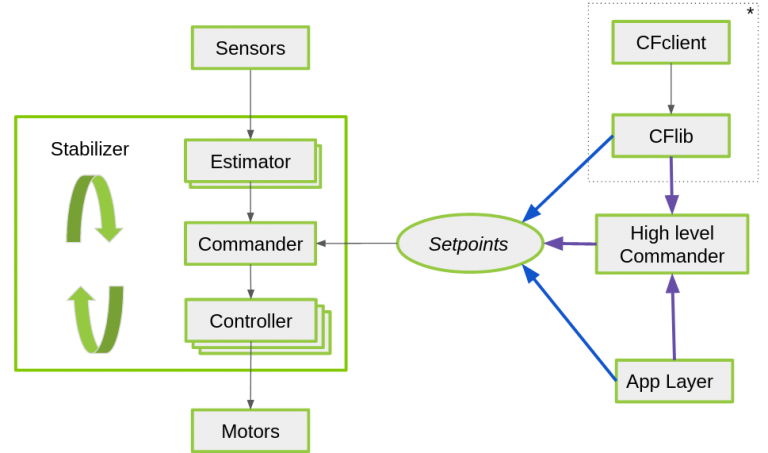
\includegraphics[width=.6\linewidth]{figures/content/chapter5/无人机飞控.png}
  \caption{无人机飞行控制的Commander模块}
  \label{fig:5_6}
  \end{figure}
Crazyflie 2.1 无人机的飞行控制模块采用基于 setpoint 的分层闭环控制架构，通过统一的目标状态描述实现上层控制输入与底层控制器之间的解耦。在该机制中，setpoint 用于描述无人机在当前时刻的期望状态，并作为控制器的参考输入，与状态估计模块输出的实际状态进行比较，从而驱动多层控制器逐级完成闭环调节。根据控制目标的不同，系统支持多种 setpoint 工作模式，包括绝对位置模式（modeAbs）、速度模式（modeVelocity）以及禁用模式（modeDisable），从而能够适应不同任务场景下的控制需求。

在本文的系统实现中，主要采用速度模式（modeVelocity）作为无人机的控制方式。在该模式下，setpoint 不再直接描述无人机的空间位置，而是以速度作为控制目标，具体包括$x$、$y$、$z$三个方向的线速度以及偏航角变化率。控制系统通过将期望速度与当前估计速度进行比较，构建速度闭环控制，并进一步生成对应的加速度指令。由于四旋翼无人机的平动控制依赖于姿态调节，系统将期望加速度转换为相应的滚转角与俯仰角设定值，随后通过姿态控制环和角速度控制环逐级实现闭环调节，最终作用于电机驱动，实现对无人机运动状态的精确控制。

相较于绝对位置模式，速度模式具有更加连续和平滑的控制特性。由于其不依赖离散的位置目标点，而是通过连续速度输入驱动无人机运动，因此能够有效避免位置控制中可能出现的震荡与突变问题。此外，速度模式对系统响应速度要求较低，控制链路更为直接，有利于提高动态响应性能。在多无人机协同控制或基于外部感知（如UWB定位）的场景中，通过直接控制速度可以更方便地实现一致性控制与分布式决策，因此具有更强的适用性。



在本系统中，H7 芯片上运行的飞行控制算法需要将控制指令（setpoint）实时传输至无人机固件执行。由于无线通信带宽受限，若每次均传输完整的 setpoint 结构体，将带来较大的通信开销。
因此，有必要对传输数据格式进行优化设计，以降低数据量并提升通信效率。

首先，通过对飞控过程中 setpoint 使用情况的分析发现，相较于默认值，每一时刻仅有部分字段发生变化。据此，本文提出一种基于“差分传输”的数据压缩方法，仅传输相对于默认 setpoint 的变化量，从而显著减少通信负载。

具体而言，设计如下差分数据结构：
\begin{lstlisting}[language=C]
struct Diff
{
    uint8_t change;
    uint8_t data[2 * SIZE_OF_SETPOINT];
};
\end{lstlisting}

其中，\texttt{change} 表示当前 setpoint 中相较默认值发生变化的字节数量；\texttt{data} 用于存储具体变化信息。对于每一个发生变化的字节，采用“位置 + 数值”的编码方式进行存储，即：
\begin{itemize}
    \item \texttt{data[2n]} 表示发生变化的字节在 setpoint 中的位置索引；
    \item \texttt{data[2n+1]} 表示该位置更新后的数值。
\end{itemize}

因此，在实际传输过程中，仅需发送 $2 \times \texttt{change} + 1$ 个字节即可完成一次 setpoint 更新，相较于原始整结构体传输方式大幅降低了数据量。

在接收端，无人机固件首先加载默认 setpoint，然后根据接收到的差分数据，对对应位置进行逐字节更新，从而恢复出完整的控制指令。

为验证该方法的有效性，本文在无人机固件中构建了“自发送”测试机制，即由系统内部模拟 H7 芯片发送飞控数据。实验结果表明，该方法能够在保证飞行控制正常执行的前提下显著降低通信开销。在一次典型飞行测试中，改进方案的数据传输总量约为原始方案的 $15.58\%$，验证了所提出方法的高效性与可行性。

\section{系统部署与运行方案}
在系统部署过程中，不同模块采用了不同的程序烧录与调试方式。对于 Crazyflie 无人机本体，其固件通过 Crazyradio PA 无线模块进行烧录，上位机经由 2.4GHz 通信链路将编译好的固件下载至无人机，实现快速更新与部署。

对于 Adhoc Deck 扩展板，其程序烧录采用 ST-Link 调试器，通过 SWD 接口将程序下载至 STM32H7 芯片中。该方式主要用于嵌入式算法与底层驱动的开发与调试。

在调试方面，Adhoc Deck 采用 SWV（Serial Wire Viewer）机制进行运行信息输出，通过调试接口实时打印关键变量与系统状态，用于辅助程序调试与功能验证。

\begin{figure}[htbp]
  \centering
  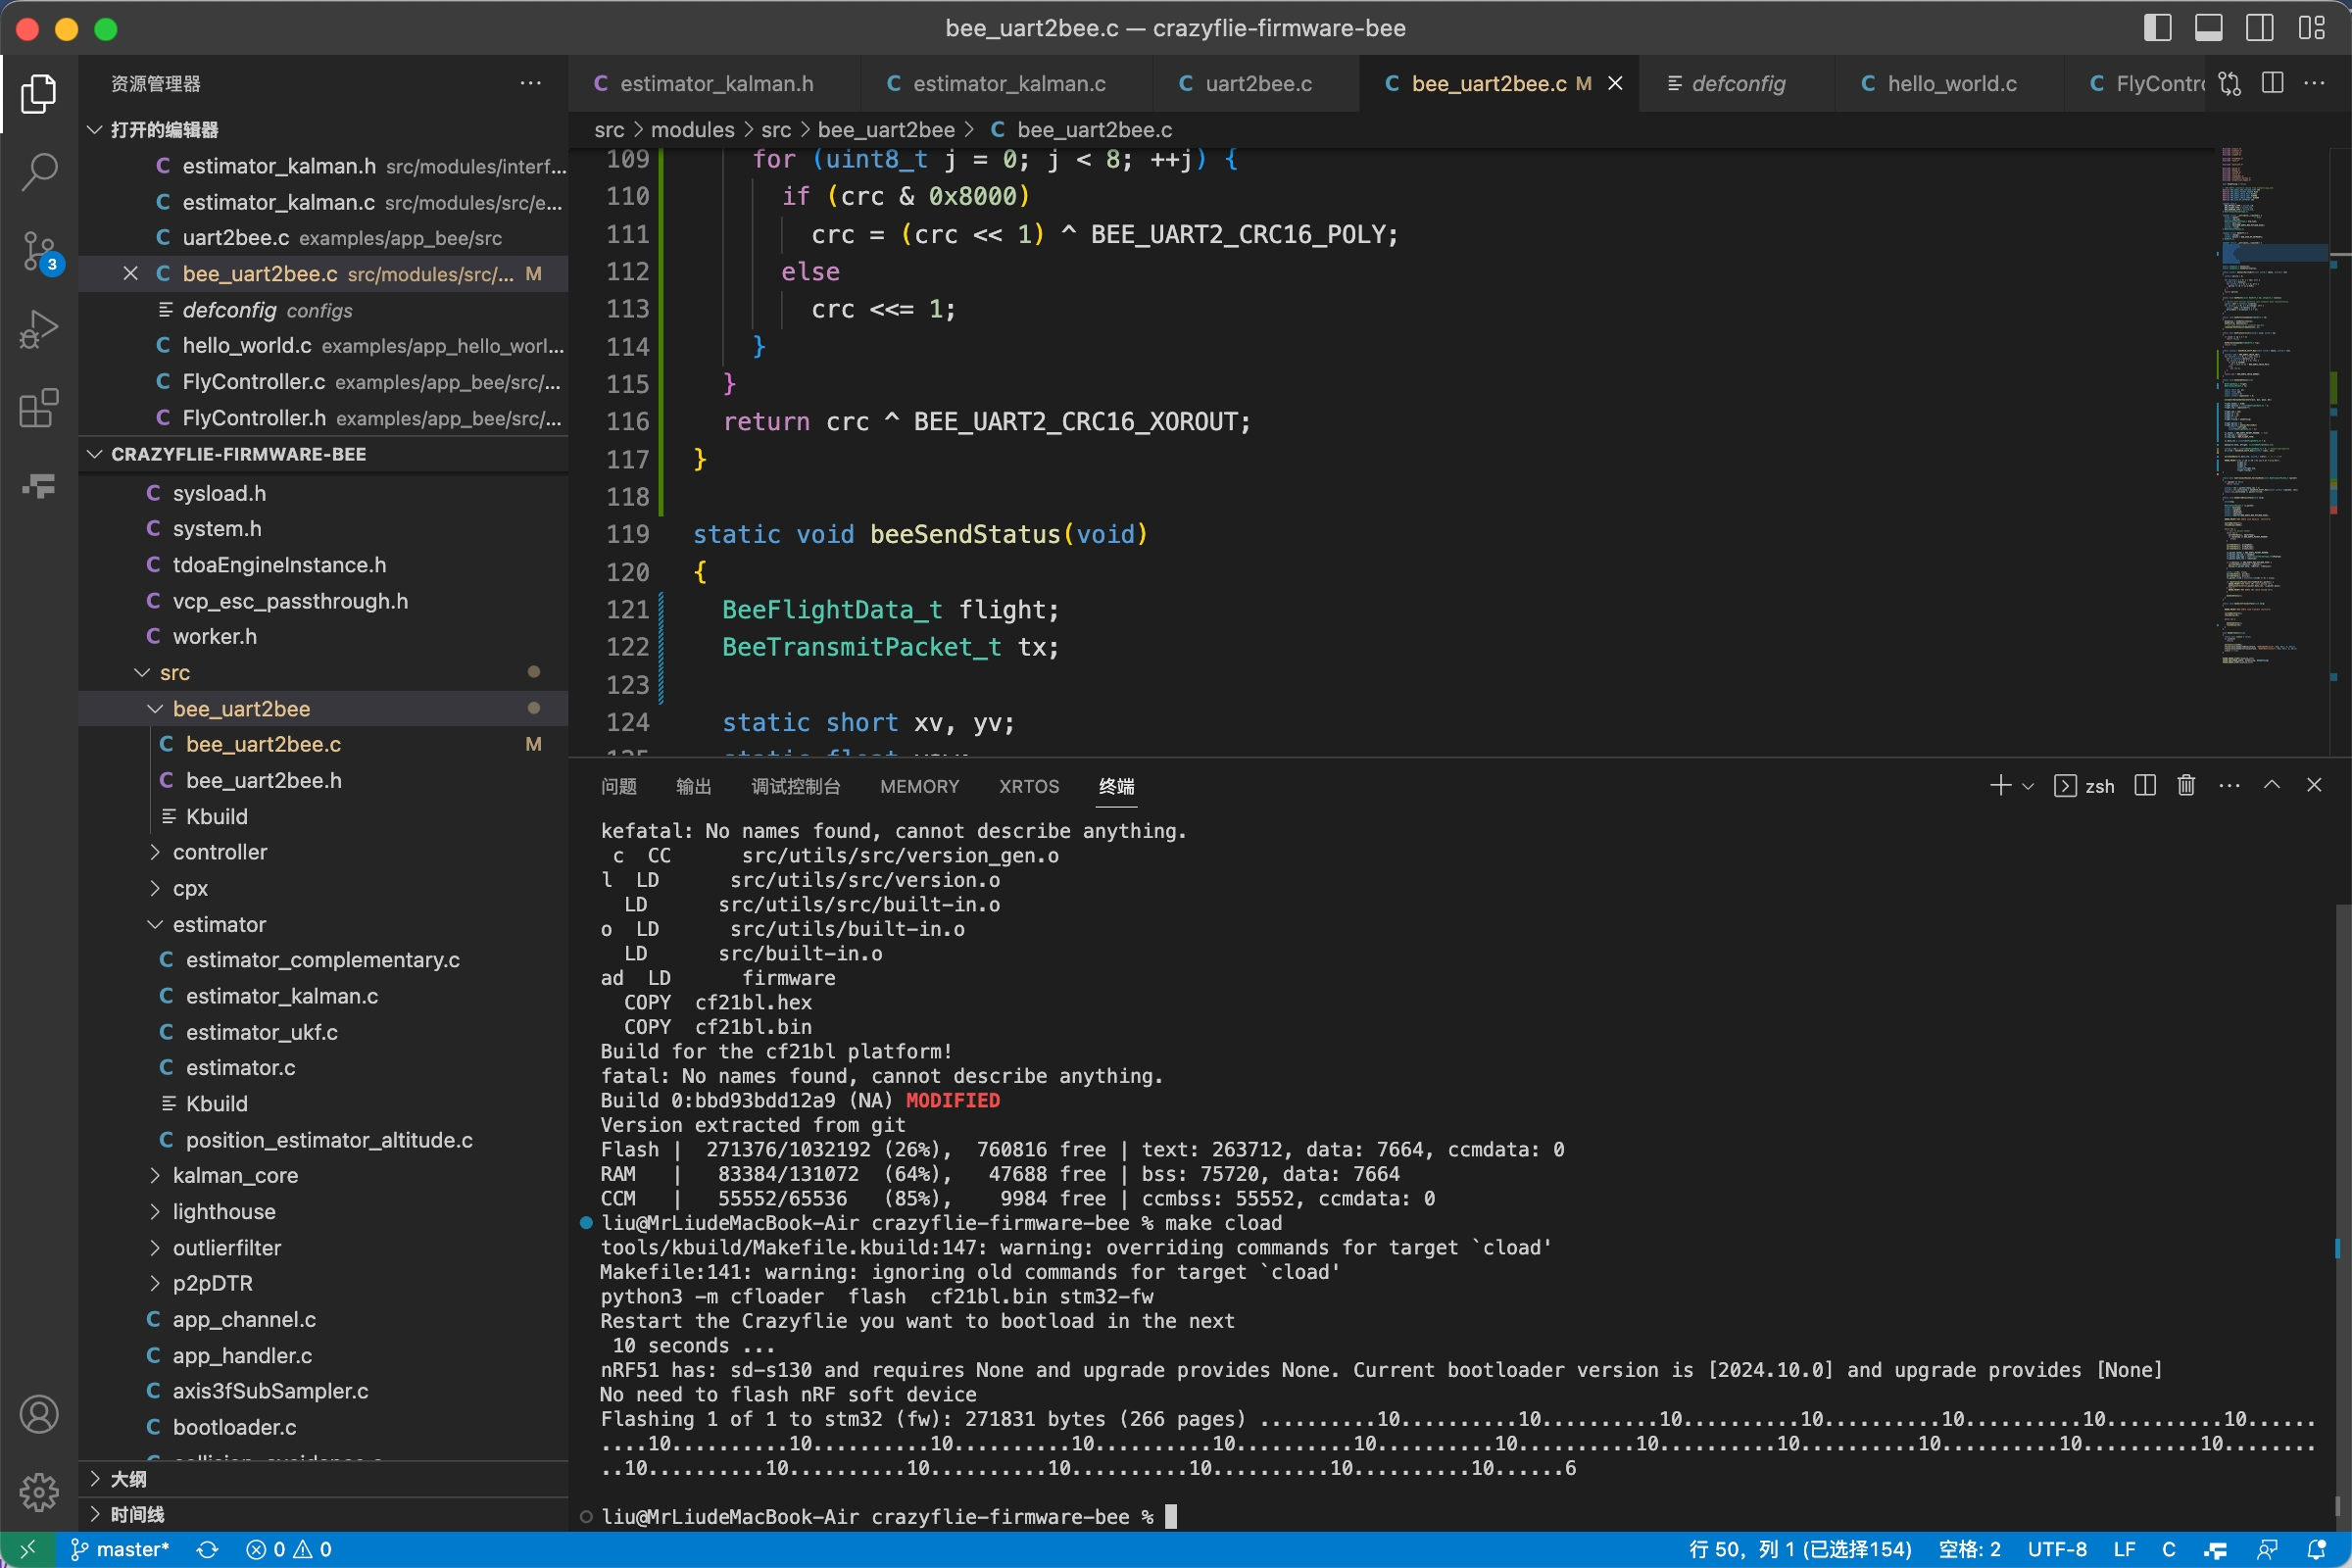
\includegraphics[width=.6\linewidth]{figures/content/chapter5/无人机编译烧录.jpg}
  \caption{无人机的编译与烧录}
  \label{fig:5_7}
\end{figure}

\begin{figure}[htbp]
  \centering
  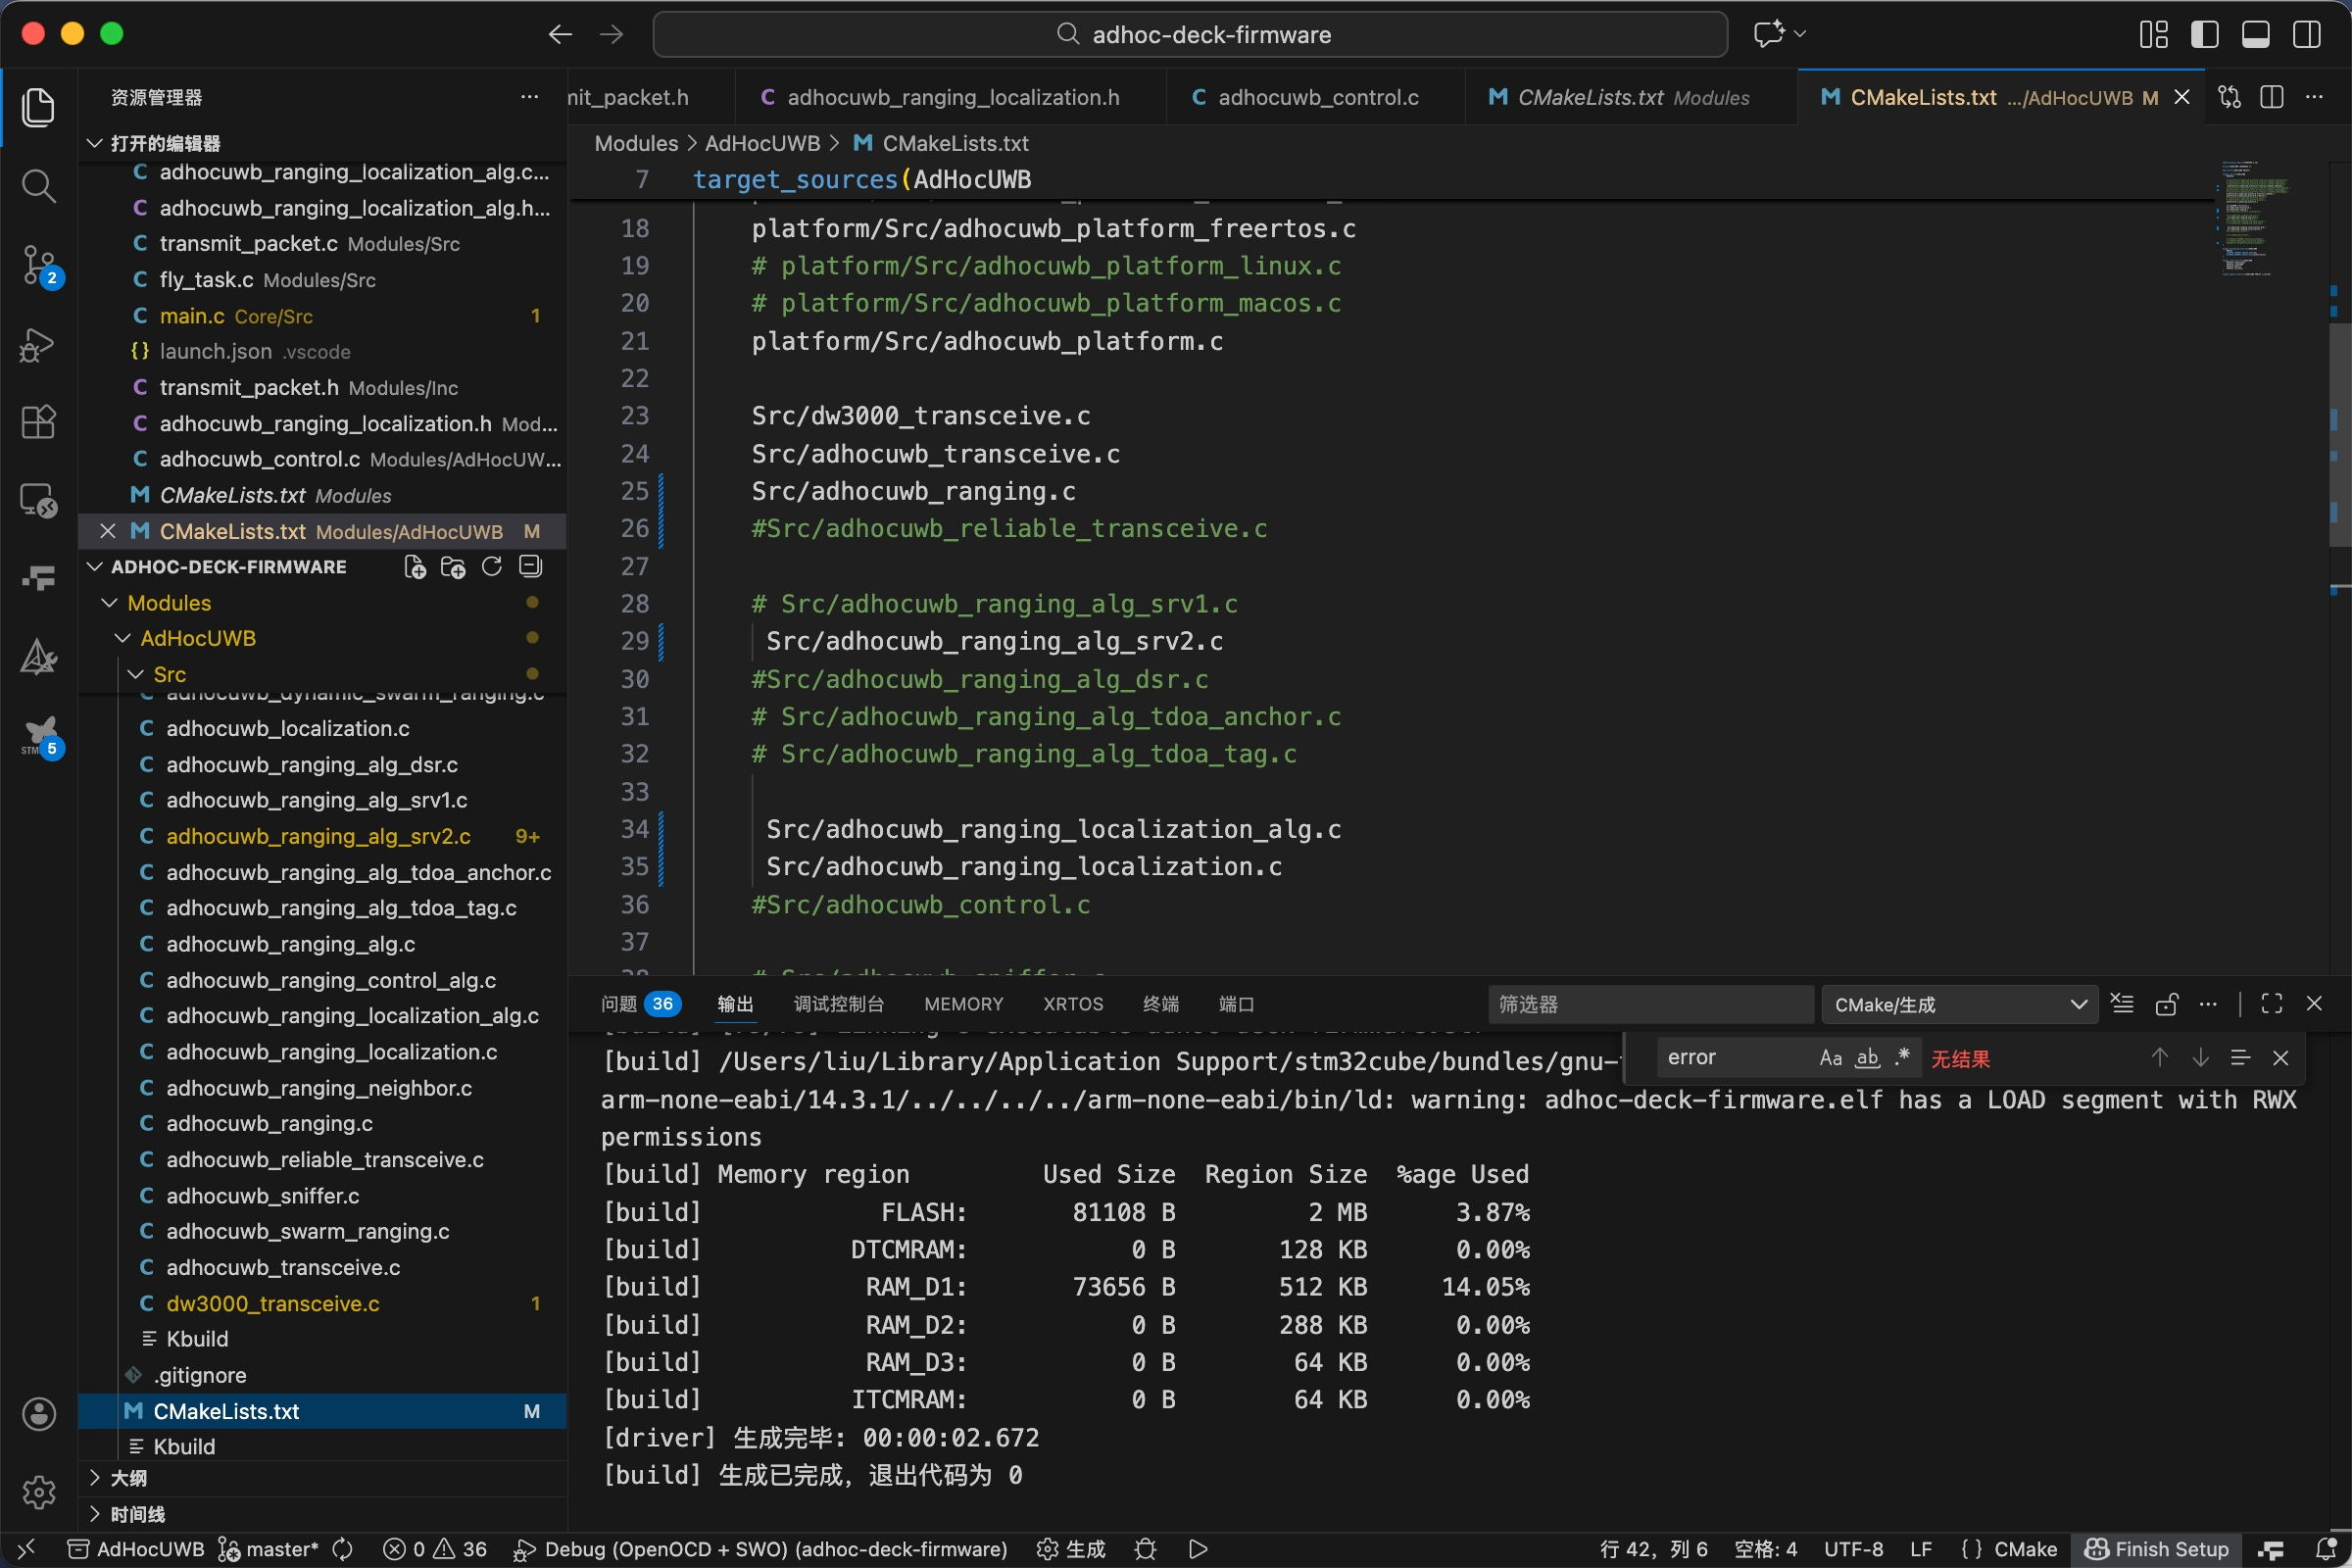
\includegraphics[width=.6\linewidth]{figures/content/chapter5/stmH7烧录.jpg}
  \caption{Adhoc Deck的编译与烧录}
  \label{fig:5_8}
\end{figure}

\begin{figure}[htbp]
  \centering
  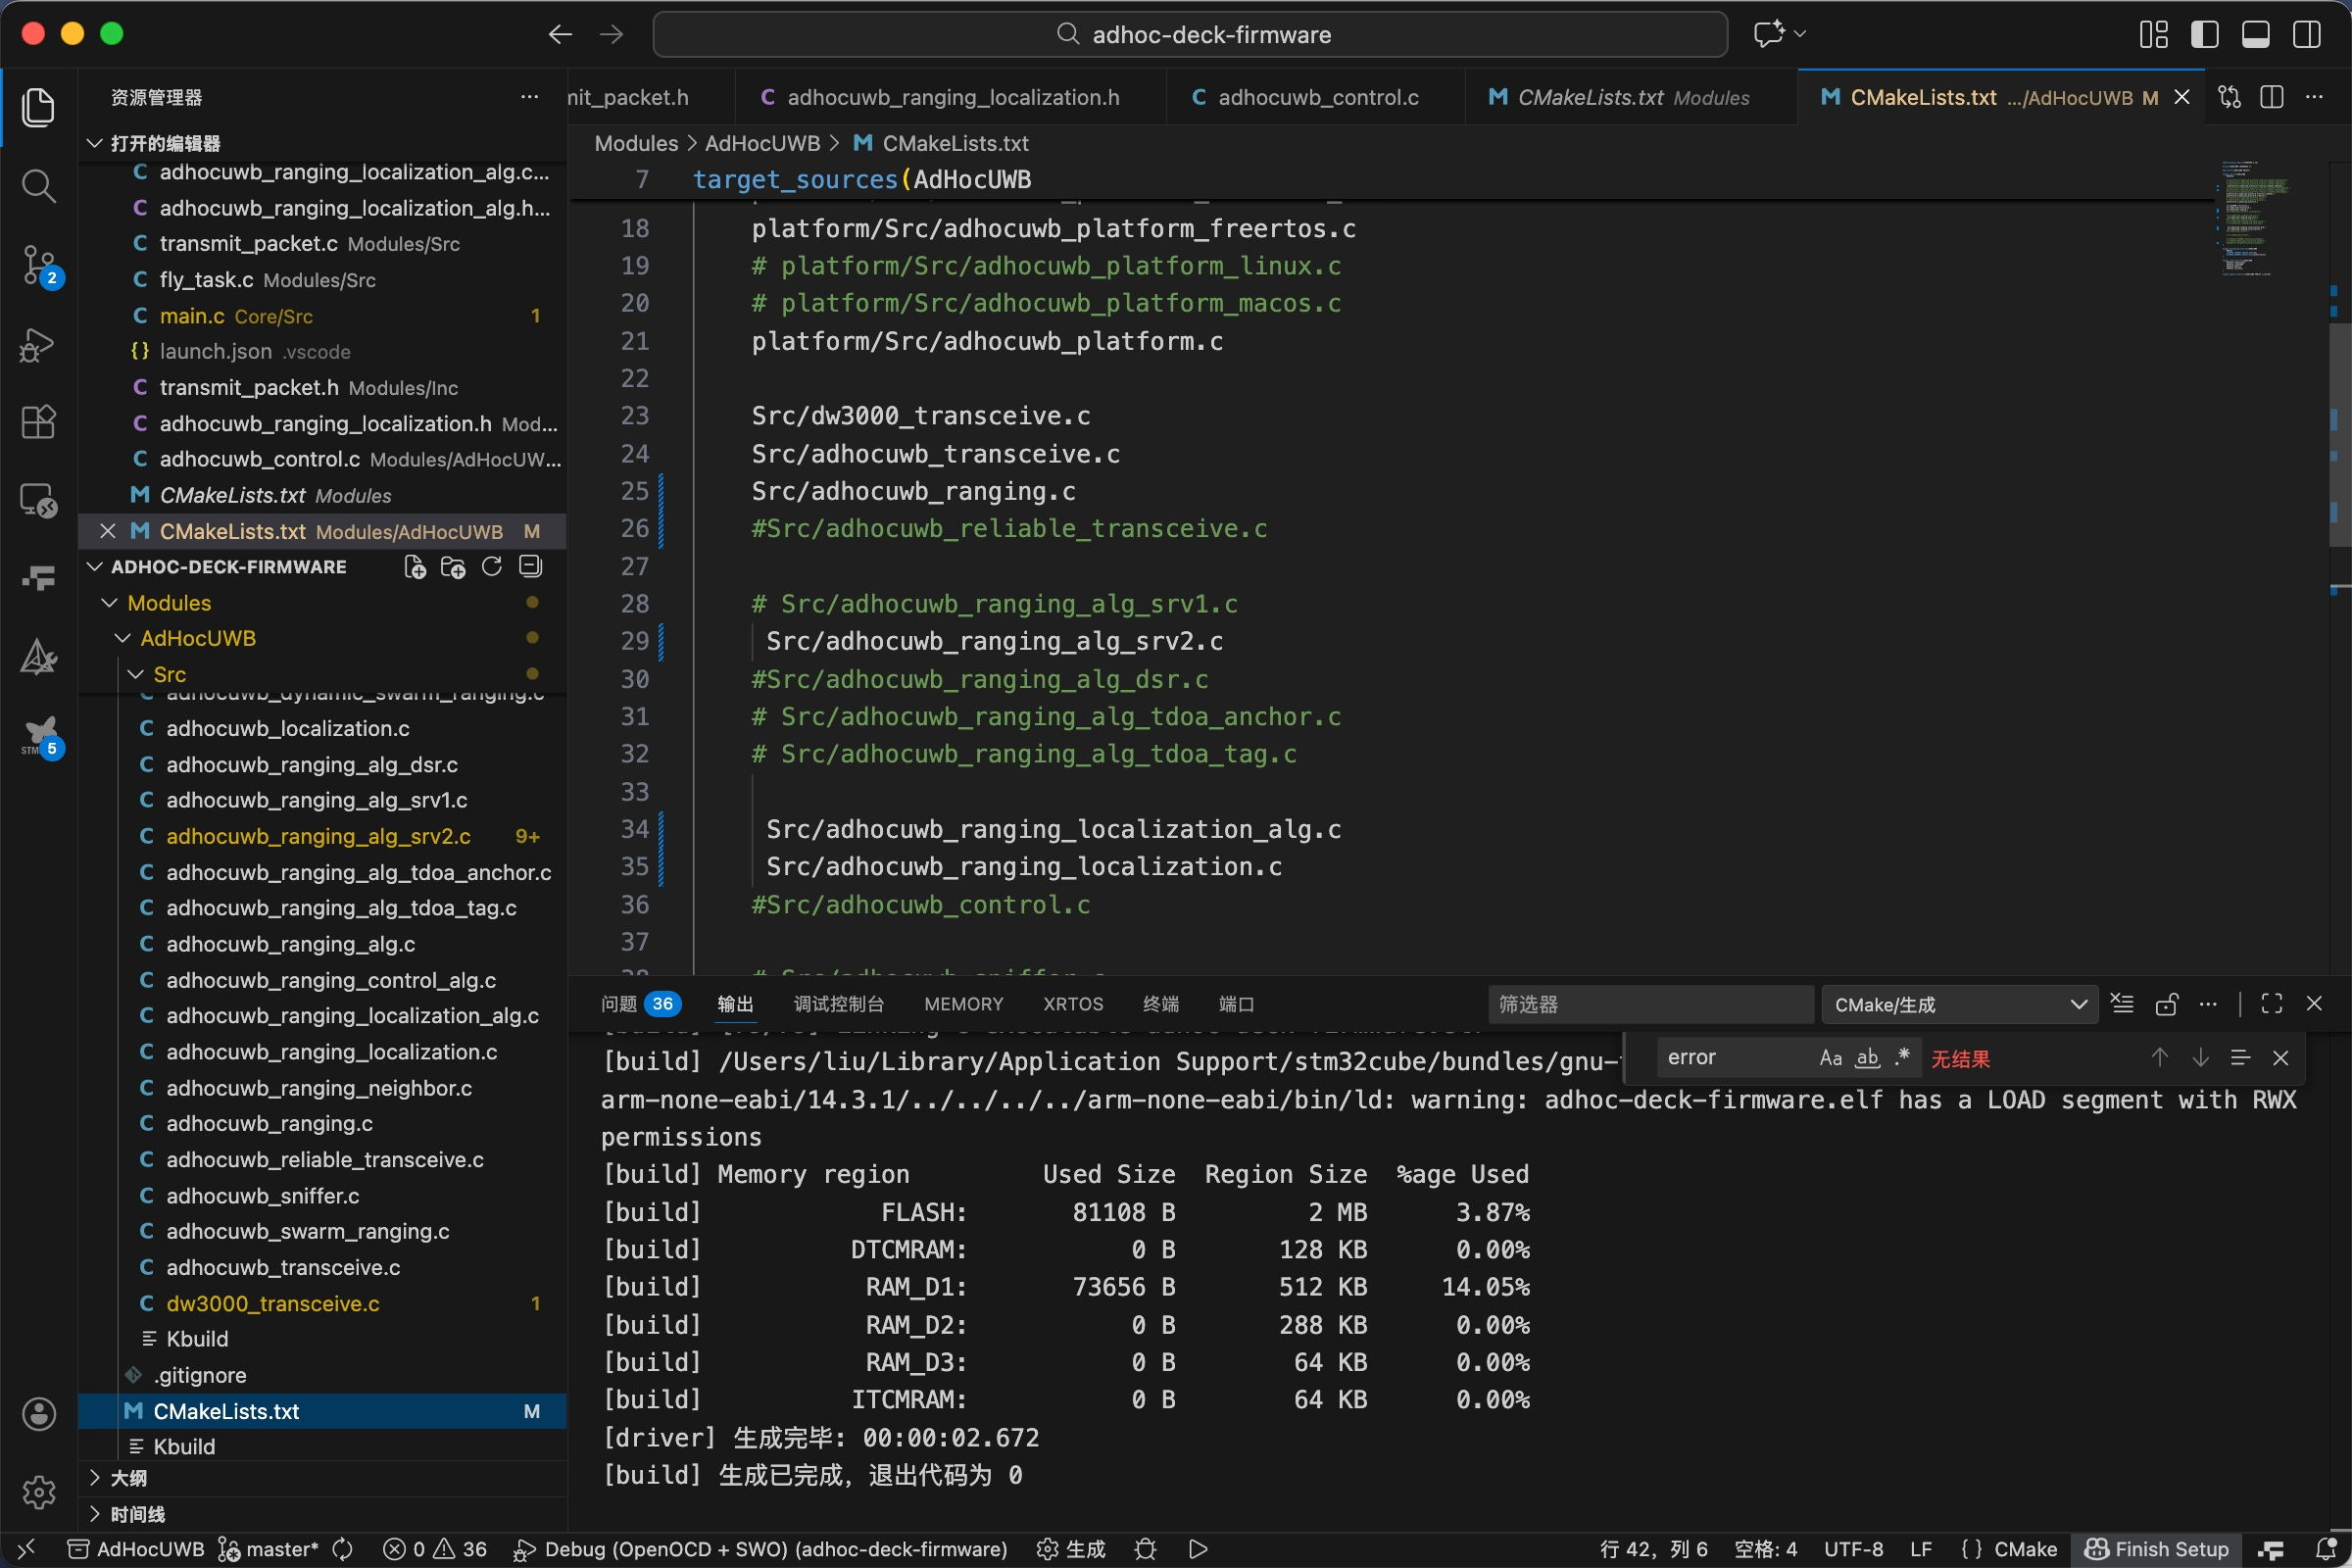
\includegraphics[width=.6\linewidth]{figures/content/chapter5/stmH7烧录.jpg}
  \caption{Adhoc Deck运行调试中的SWV输出}
  \label{fig:5_9}
\end{figure}
\section{ 系统测试与运行结果} 
%无人机编队飞行图以及Deck展示图

\section{本章小结} 

本章围绕微型无人机集群测距与自主导航原型系统的设计与实现，系统性地完成了从硬件构建到软件集成，再到实际飞行验证的整体工作，实现了前文算法研究向工程应用的有效落地。

在硬件方面，构建了由外部监控平台、领航无人机与跟随无人机组成的集群系统架构。通过集成 UWB 测距模块、光流与多方向距离传感器以及动捕系统，实现了多源信息融合的感知与定位能力，为集群协同提供了可靠的数据基础。
在软件方面，设计了分层模块化的软件架构，将系统划分为单机功能模块、集群协同模块以及算法支撑模块。针对领航与跟随两类无人机的不同功能需求，分别构建了自主导航、协同定位与局部避障等关键模块，并通过统一的数据流实现“感知—定位—决策—控制”的闭环运行机制。同时，结合 CRTP 通信协议与基于 UART 的高效数据传输机制，保障了系统在多节点协同下的实时性与稳定性。

在系统部署与实验验证方面，完成了无人机固件与嵌入式平台的编译烧录与调试，构建了真实飞行实验环境。实验结果表明，所设计的原型系统能够在资源受限的微型无人机平台上稳定运行，实现多无人机之间的可靠测距与协同定位，并支持领航—跟随模式下的自主导航与避障飞行，验证了本文所提方法在实际复杂环境中的可行性与有效性。


